\documentclass[border=10pt]{standalone}

\usepackage{tikz}
\usepackage{tikzsymbols}
\usetikzlibrary{calc,patterns,shapes.geometric}

\def\centerarc[#1](#2)(#3:#4:#5){\draw[#1] ($(#2)+({#5*cos(#3)},{#5*sin(#3)})$) arc (#3:#4:#5);}

\begin{document}
	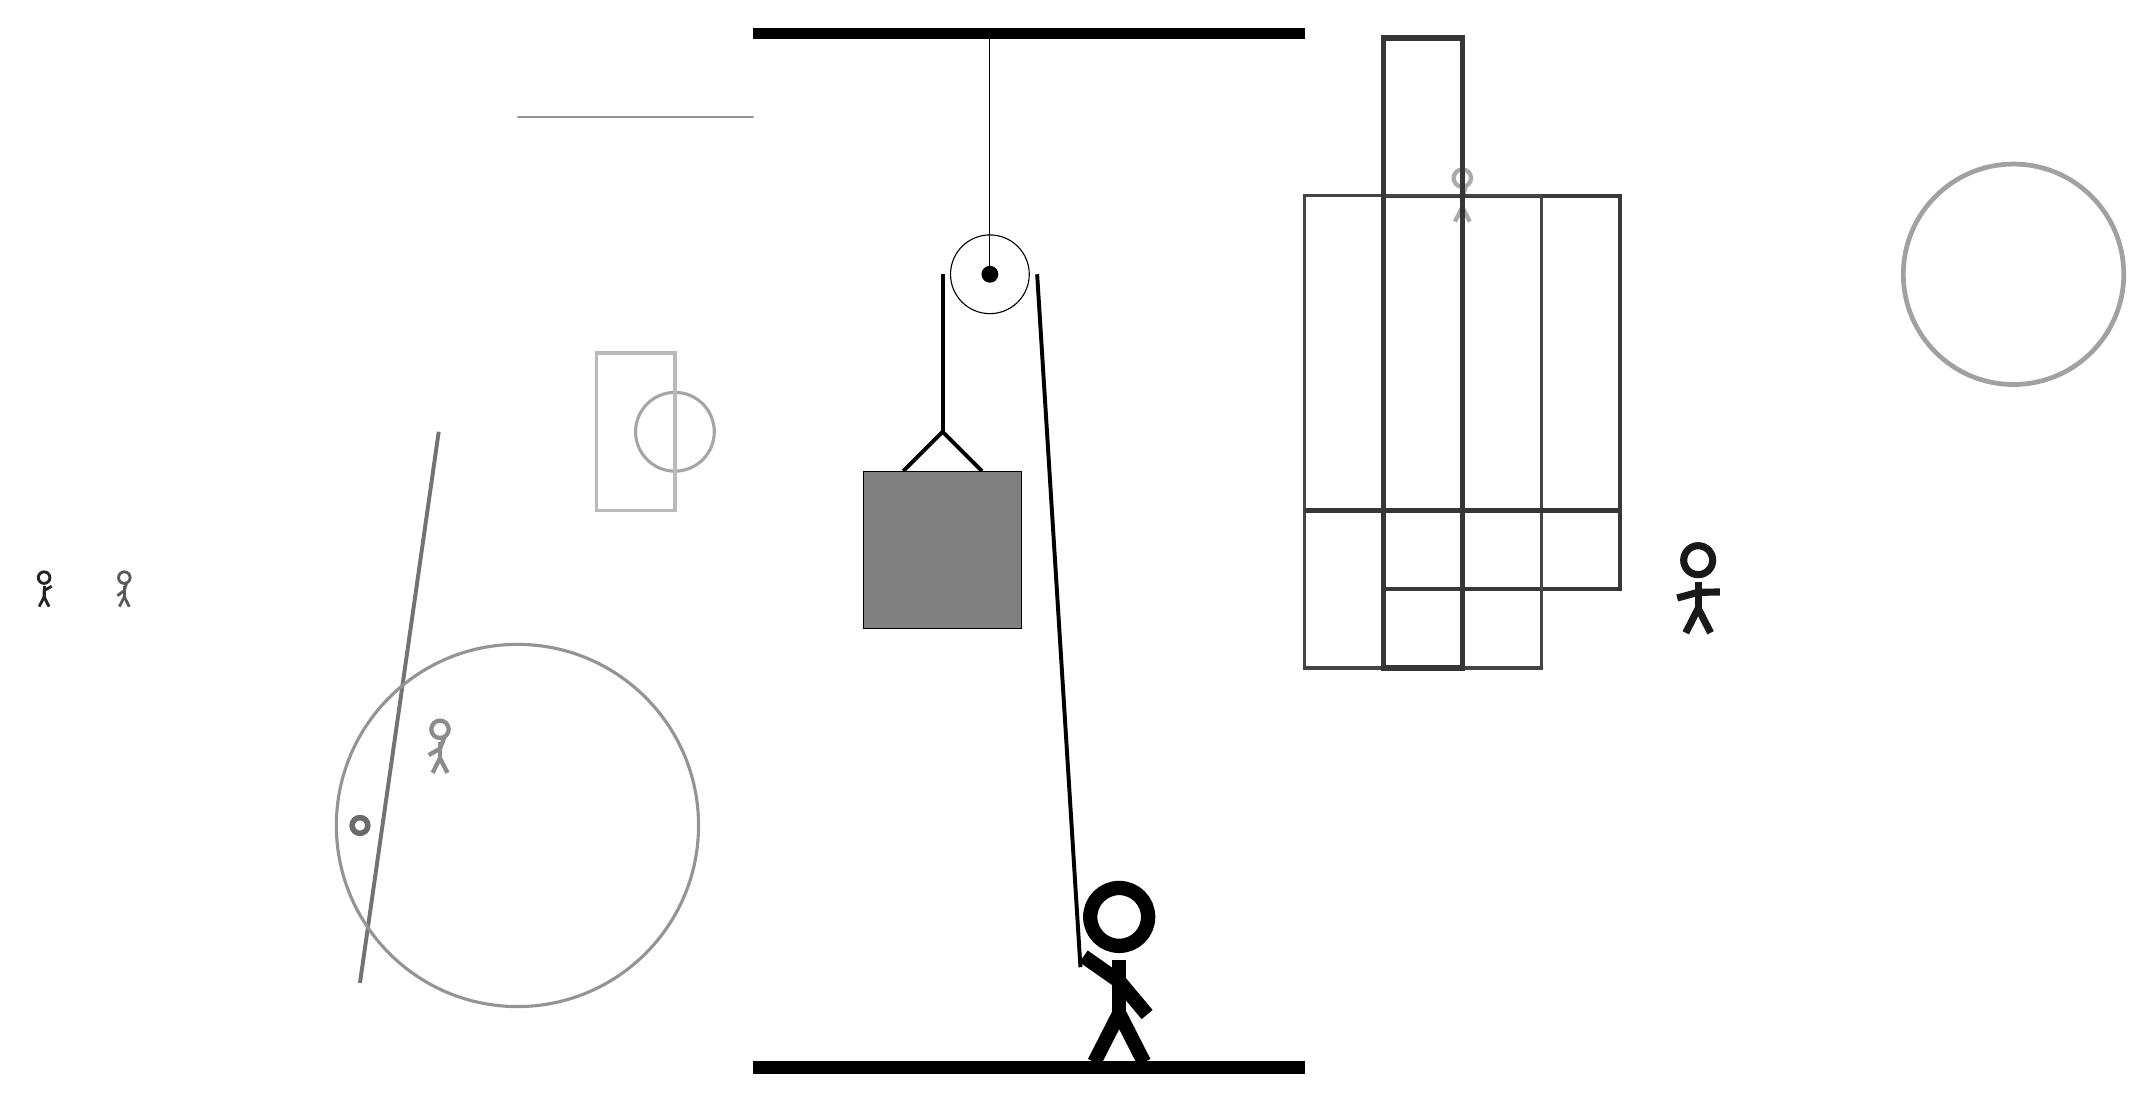
\begin{tikzpicture}
		%%%%% START %%%%%
		
		\draw[fill=black] (-2, 10) rectangle (5, 10.125);
		
		\draw (1, 7) circle (0.5);
		\draw[fill=black] (1, 7) circle (0.1);
		\draw (1, 10) -- (1, 7);
		
		\draw[line width=0.5mm] (-0.1, 4.5) -- (0.4, 5.0) -- (0.9, 4.5);
		\draw[fill=black!50] (-0.6, 4.5) rectangle (1.4, 2.5);
		
		\draw[line width=0.5mm] (0.4, 7) -- (0.4, 5.0);
		\centerarc[line width=0.5mm](1, 7)(0:180:0.6);
		\draw[line width=0.5mm](1.6, 7) -- (2.15, -1.8);
		
		\node at (2.6, -1.9) {\Strichmaxerl[10][-35][-50]};
		
		\draw [line width=0.7mm, color=black!58](-7, 0) circle (0.1);
		
		\draw[line width=0.2mm, color=black!41] (-2, 9) rectangle (-5, 9);
		\draw[line width=0.5mm, color=black!55](-6, 5) -- (-7, -2);
		\node[line width=0.5mm, color=black!45] at (-6, 1) {\Strichmaxerl[3][30][69]};
		\draw [line width=0.4mm, color=black!35](-3, 5) circle (0.5);
		\draw[line width=0.4mm, color=black!27] (-3, 6) rectangle (-4, 4);
		\node[line width=0.6mm, color=black!33] at (7, 8) {\Strichmaxerl[3][89][72]};
		\draw[line width=0.5mm, color=black!78] (6, 8) rectangle (9, 3);
		\draw [line width=0.4mm, color=black!42](-5, 0) circle (2.3);
		
		\draw [line width=0.6mm, color=black!37](14, 7) circle (1.4);
		\draw[line width=0.4mm, color=black!73] (5, 8) rectangle (8, 2);
		\draw[line width=0.7mm, color=black!79] (6, 10) rectangle (7, 2);
		\node[line width=0.7mm, color=black!65] at (-10, 3) {\Strichmaxerl[2][37][73]};
		
		\draw[line width=0.6mm, color=black!79] (5, 4) rectangle (9, 4);
		\node[line width=0.5mm, color=black!86] at (-11, 3) {\Strichmaxerl[2][89][29]};
		\node[line width=0.5mm, color=black!90] at (10, 3) {\Strichmaxerl[5][15][1]};
		
		\draw[fill=black] (-2, -3) rectangle (5, -3.15);
		
		%%%%% END %%%%%
	\end{tikzpicture}
\end{document}